\phantomsection
\section*{Chapter 5}
\addcontentsline{toc}{section}{Chapter 5}

\subsection*{5.2}

\begin{figure}[H]
  \centering
  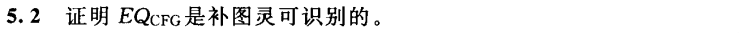
\includegraphics[width=0.8\textwidth]{chapters/imgs/hw_5_2.png}
  \caption{}
  \label{fig:hw_5_2}
\end{figure}

证明。要证明
\[
    \mathrm{EQ}_{\mathrm{CFG}}
\]
是 co-Turing-recognizable，只需证明它的补语言
\[
    \overline{\mathrm{EQ}_{\mathrm{CFG}}}
    =\{\langle G,H\rangle\mid L(G)\ne L(H)\}
\]
是 Turing-recognizable。

\medskip
构造识别器 $R$ 如下。在输入
\[
    \langle G,H\rangle
\]
上，枚举所有字符串
\[
    w_1,w_2,w_3,\dots
\]
并对每个 $w_i$ 测试：

\medskip
\noindent
1. 是否
\[
    w_i\in L(G);
\]

\medskip
\noindent
2. 是否
\[
    w_i\in L(H).
\]

\medskip
因为 CFG 的成员资格问题是可判定的，所以这两个测试都能停机。若发现某个 $w_i$ 满足
\[
    w_i\in L(G)\setminus L(H)
    \qquad\text{或}\qquad
    w_i\in L(H)\setminus L(G),
\]
就接受。

\medskip
若
\[
    L(G)\ne L(H),
\]
则它们的对称差非空，故必存在某个字符串最终会被枚举到并使 $R$ 接受。若
\[
    L(G)=L(H),
\]
则 $R$ 永不接受。

因此
\[
    \overline{\mathrm{EQ}_{\mathrm{CFG}}}
\]
是 Turing-recognizable，从而
\[
    \mathrm{EQ}_{\mathrm{CFG}}
\]
是 co-Turing-recognizable。$\blacksquare$

\paragraph{解释.}
“两个 CFG 不相等”只要找到一个见证串即可。因为 CFG 成员资格可判定，我们可以把所有字符串逐个检验；一旦发现落在对称差中的字符串，就识别出了补语言。

\subsection*{5.5}

\begin{figure}[H]
  \centering
  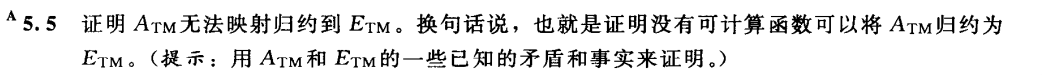
\includegraphics[width=0.8\textwidth]{chapters/imgs/hw_5_5.png}
  \caption{}
  \label{fig:hw_5_5}
\end{figure}

证明。反设存在一个可计算函数 $f$，把
\[
    A_{\mathrm{TM}}
\]
映射归约到
\[
    E_{\mathrm{TM}}.
\]
也就是说，对任意输入 $x$，
\[
    x\in A_{\mathrm{TM}}
    \iff
    f(x)\in E_{\mathrm{TM}}.
\]

\medskip
记
\[
    \overline{E_{\mathrm{TM}}}
    =
    \{\langle M\rangle\mid L(M)\ne\varnothing\}.
\]
这个语言是 Turing-recognizable。设图灵机 $R$ 识别
\[
    \overline{E_{\mathrm{TM}}}.
\]
我们构造图灵机 $S$ 来识别
\[
    \overline{A_{\mathrm{TM}}}
\]
如下：

\begin{myalgo}{构造的图灵机 $S$}
\begin{algorithmic}[1]
  \Require 输入 $x$
  \Ensure 若 $x\in \overline{A_{\mathrm{TM}}}$ 则接受；否则不接受
  \State 计算 $f(x)$
  \State 在输入 $f(x)$ 上运行 $R$
  \If{$R$ 接受}
    \State \textbf{接受}
  \EndIf
\end{algorithmic}
\end{myalgo}

\medskip
下面验证 $S$ 的正确性。对任意输入 $x$，
\[
    x\in \overline{A_{\mathrm{TM}}}
    \iff
    x\notin A_{\mathrm{TM}}
    \iff
    f(x)\notin E_{\mathrm{TM}}
    \iff
    f(x)\in \overline{E_{\mathrm{TM}}}.
\]
因此，若
\[
    x\in \overline{A_{\mathrm{TM}}},
\]
则 $R$ 接受 $f(x)$，故 $S$ 接受；若
\[
    x\notin \overline{A_{\mathrm{TM}}},
\]
则 $R$ 不会接受 $f(x)$，故 $S$ 也不接受。于是 $S$ 识别了
\[
    \overline{A_{\mathrm{TM}}}.
\]

\medskip
这与已知结论矛盾，因为
\[
    \overline{A_{\mathrm{TM}}}
\]
不是 Turing-recognizable。

故不存在这样的可计算函数 $f$。因此
\[
    A_{\mathrm{TM}}\not\le_m E_{\mathrm{TM}}.
\]
$\blacksquare$

\paragraph{解释.}
这题不是说两个语言都不可判定，就一定不能归约；关键在于它们的“可识别方向”不同。$E_{\mathrm{TM}}$ 是 co-Turing-recognizable，而 $A_{\mathrm{TM}}$ 不是；如果真能把 $A_{\mathrm{TM}}$ 归约到 $E_{\mathrm{TM}}$，补语言的可识别性就会被错误地传回去。

\subsection*{5.9}

\begin{figure}[H]
  \centering
  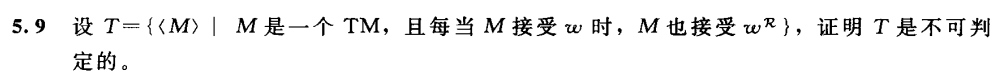
\includegraphics[width=0.8\textwidth]{chapters/imgs/hw_5_9.png}
  \caption{}
  \label{fig:hw_5_9}
\end{figure}

证明。反设存在图灵机 $R$ 判定
\[
    \mathrm{AMBIG}_{\mathrm{CFG}}
    =\{\langle G\rangle\mid G\text{ 是二义的 CFG}\}.
\]
我们构造图灵机 $S$ 来判定 PCP。

\begin{myalgo}{构造的图灵机 $S$}
\begin{algorithmic}[1]
  \Require PCP 实例 $P=\bigl(\langle t_1,b_1\rangle,\langle t_2,b_2\rangle,\dots,\langle t_k,b_k\rangle\bigr)$
  \Ensure 若 $P$ 有解则接受；否则拒绝
  \State 引入新的终结符 $a_1,\dots,a_k$
  \State 构造文法 $G$，其中
  \[
      S\to T\mid B,
  \]
  \[
      T\to t_1Ta_1\mid\cdots\mid t_kTa_k\mid t_1a_1\mid\cdots\mid t_ka_k,
  \]
  \[
      B\to b_1Ba_1\mid\cdots\mid b_kBa_k\mid b_1a_1\mid\cdots\mid b_ka_k.
  \]
  \State 在输入 $\langle G\rangle$ 上运行 $R$
  \If{$R$ 接受}
    \State \textbf{接受}
  \Else
    \State \textbf{拒绝}
  \EndIf
\end{algorithmic}
\end{myalgo}

\medskip
下面证明 $S$ 的正确性。先证：若该 PCP 实例有解，则 $G$ 二义。设
\[
    i_1i_2\cdots i_m
\]
是一个解，即
\[
    t_{i_1}t_{i_2}\cdots t_{i_m}
    =
    b_{i_1}b_{i_2}\cdots b_{i_m}.
\]
则同一个字符串
\[
    x=
    t_{i_1}t_{i_2}\cdots t_{i_m}a_{i_m}\cdots a_{i_2}a_{i_1}
\]
可由 $T$ 推导：
\[
    T\Rightarrow t_{i_1}Ta_{i_1}
    \Rightarrow \cdots
    \Rightarrow t_{i_1}\cdots t_{i_m}a_{i_m}\cdots a_{i_1},
\]
也可由 $B$ 推导：
\[
    B\Rightarrow b_{i_1}Ba_{i_1}
    \Rightarrow \cdots
    \Rightarrow b_{i_1}\cdots b_{i_m}a_{i_m}\cdots a_{i_1}.
\]
因为顶串与底串相等，这两个结果是同一个字符串 $x$。于是
\[
    S\Rightarrow T\Rightarrow^* x
    \qquad\text{且}\qquad
    S\Rightarrow B\Rightarrow^* x,
\]
故 $G$ 二义，因此 $R$ 接受 $\langle G\rangle$，从而 $S$ 接受该 PCP 实例。

\medskip
再证：若 $G$ 二义，则该 PCP 实例有解。

注意，$T$ 和 $B$ 各自都是无二义的。因为任何由它们生成的字符串末尾都含有一个由
\[
    a_{i_m}\cdots a_{i_1}
\]
构成的后缀，而这段后缀唯一确定了所选取的指标序列
\[
    i_1,\dots,i_m.
\]
一旦指标序列确定，前面的部分也就唯一确定。因此，一个字符串若有两种不同推导，只能是其中一种从
\[
    S\to T
\]
开始，另一种从
\[
    S\to B
\]
开始。

于是存在某个字符串 $x$，既在 $L(T)$ 中，又在 $L(B)$ 中。由末尾的
\[
    a_{i_m}\cdots a_{i_1}
\]
可知，这两种推导使用的是同一个指标序列
\[
    i_1,\dots,i_m.
\]
因此
\[
    t_{i_1}\cdots t_{i_m}
    =
    b_{i_1}\cdots b_{i_m},
\]
即该 PCP 实例有解。于是 $R$ 接受 $\langle G\rangle$ 当且仅当输入 PCP 实例有解。

\medskip
因此，若 $R$ 存在，则 $S$ 判定 PCP，这与 PCP 不可判定矛盾。故
\[
    \mathrm{AMBIG}_{\mathrm{CFG}}
\]
不可判定。$\blacksquare$

\paragraph{解释.}
这个归约的核心是把“同一指标序列”编码在尾部的
\[
    a_{i_m}\cdots a_{i_1}
\]
里。于是，若同一个字符串既能从 $T$ 生成又能从 $B$ 生成，就意味着同一串牌在顶部和底部拼出的结果相同，这正是 PCP 解。

\subsection*{5.13}

\begin{figure}[H]
  \centering
  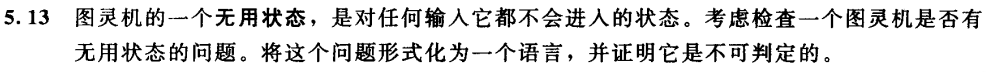
\includegraphics[width=0.8\textwidth]{chapters/imgs/hw_5_13.png}
  \caption{}
  \label{fig:hw_5_13}
\end{figure}

取
\[
    B=A_{\mathrm{TM}}.
\]
这是一个不可判定语言。

\medskip
定义可计算函数
\[
    f(x)=x.
\]
显然对任意 $x$，
\[
    x\in B
    \iff
    f(x)\in B.
\]
因此
\[
    B\le_m B.
\]

所以 $B=A_{\mathrm{TM}}$ 就是所要求的例子。$\blacksquare$

\subsection*{5.17}

\begin{figure}[H]
  \centering
  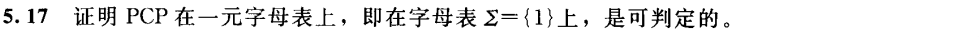
\includegraphics[width=0.8\textwidth]{chapters/imgs/hw_5_17.png}
  \caption{}
  \label{fig:hw_5_17}
\end{figure}

证明。Problem 5.16（Rice 定理）的两个条件分别是：

\medskip
\noindent
1. $P$ 是非平凡的，即它既不为空，也不包含所有图灵机描述；

\medskip
\noindent
2. $P$ 只取决于图灵机所识别的语言，即若
\[
    L(M_1)=L(M_2),
\]
则
\[
    \langle M_1\rangle\in P
    \iff
    \langle M_2\rangle\in P.
\]

\medskip
下面分别说明这两个条件都必不可少。

\paragraph{(1) 非平凡性是必要的}
若去掉“非平凡”条件，取
\[
    P=\varnothing
\]
或
\[
    P=\{\langle M\rangle\mid M\text{ 是图灵机}\},
\]
则 $P$ 显然是可判定的。前者总是拒绝，后者总是接受。因此，若不要求非平凡，就不能推出 $P$ 不可判定。

\paragraph{(2) “只取决于语言”这一条件是必要的}
若去掉第二个条件，可以取一个非平凡但与语言无关的可判定性质，例如
\[
    P=\{\langle M\rangle\mid \langle M\rangle\text{ 的长度为偶数}\}.
\]
这个 $P$ 显然是非平凡的：有些机器描述长度为偶数，有些为奇数；同时 $P$ 也是可判定的，因为只需检查输入描述的长度奇偶性。

但这个性质并不只取决于语言，因为完全可能存在
\[
    L(M_1)=L(M_2)
\]
而
\[
    |\langle M_1\rangle|
\]
与
\[
    |\langle M_2\rangle|
\]
奇偶不同。

\medskip
因此，Rice 定理中的两个条件都不能删去。$\blacksquare$

\paragraph{解释.}
Rice 定理的力量来自两个限制同时成立：它讨论的是“真正关于语言本身的性质”，而且这个性质不是恒真也不是恒假。少了任何一个条件，问题都可能退化成一个简单的可判定性质。

\subsection*{5.21}

\begin{figure}[H]
  \centering
  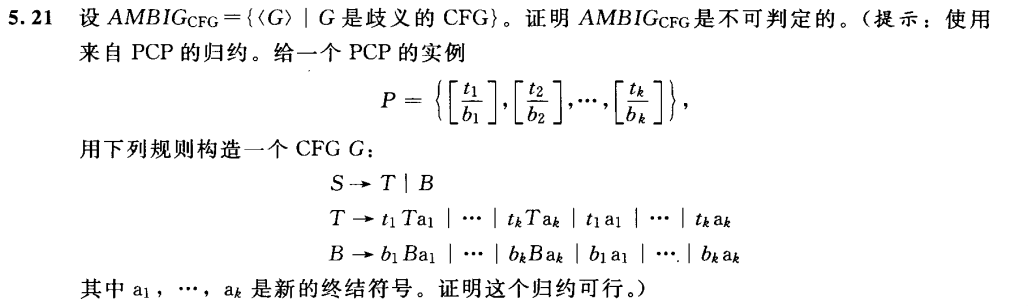
\includegraphics[width=0.8\textwidth]{chapters/imgs/hw_5_21.png}
  \caption{}
  \label{fig:hw_5_21}
\end{figure}

证明。设
\[
    \mathrm{DUP}_{\mathrm{PDA}}
    =
    \{\langle P\rangle\mid P\text{ 是 PDA 且 }L(P)\cap\{ww\mid w\in\{0,1\}^*\}\ne\varnothing\}.
\]
我们用 computation history method 证明它不可判定。反设存在图灵机 $R$ 判定
\[
    \mathrm{DUP}_{\mathrm{PDA}}.
\]

\medskip
我们构造图灵机 $S$ 来判定
\[
    A_{\mathrm{TM}}
\]
如下。给定输入
\[
    \langle M,w\rangle,
\]
$S$ 将构造一个 PDA $P_{M,w}$，再把它交给 $R$。

\medskip
首先回忆接受计算历史。若 $M$ 在输入 $w$ 上接受，则存在一串配置
\[
    C_1,C_2,\dots,C_m,
\]
其中 $C_1$ 是初始配置，$C_m$ 是接受配置，且每个 $C_{i+1}$ 都是 $C_i$ 的合法后继。

\medskip
考虑如下编码：
\[
    x=C_1\#C_2^R\#C_3\#C_4^R\#\cdots,
\]
即把偶数项配置反转后插入分隔符 $\#$。

\medskip
定义两个语言：

\medskip
\noindent
$A_{M,w}$：所有上述形式的字符串 $x$，满足
\[
    C_1
\]
是 $M$ 在 $w$ 上的初始配置，
\[
    C_m
\]
是接受配置，并且每一对奇偶相邻配置
\[
    (C_1,C_2),\ (C_3,C_4),\dots
\]
都是合法一步转移；

\medskip
\noindent
$B_{M,w}$：所有上述形式的字符串 $x$，满足相同的首尾条件，并且每一对偶奇相邻配置
\[
    (C_2,C_3),\ (C_4,C_5),\dots
\]
都是合法一步转移。

\medskip
由于相邻的两项中恰有一项被反转，PDA 可以把其中一项压栈，再逐符号比较另一项，从而检查某一对配置是否满足合法转移关系。因此
\[
    A_{M,w}
\]
和
\[
    B_{M,w}
\]
都是上下文无关语言。

\medskip
并且
\[
    M\text{ 接受 }w
    \iff
    A_{M,w}\cap B_{M,w}\ne\varnothing.
\]
这是 computation history method 的标准结论：一个串同时通过“奇数步检查”和“偶数步检查”，当且仅当它编码了一条完整的接受计算历史。

\medskip
现在引入一个新符号 $\$$，它不出现在配置编码中。构造上下文无关语言
\[
    L_{M,w}
    =
    \{x\$y\$\mid x\in A_{M,w},\ y\in B_{M,w}\}.
\]
因为上下文无关语言对连接封闭，所以 $L_{M,w}$ 由某台 PDA $P_{M,w}$ 识别。

\begin{myalgo}{构造的图灵机 $S$}
\begin{algorithmic}[1]
  \Require 输入 $\langle M,w\rangle$
  \Ensure 若 $\langle M,w\rangle\in A_{\mathrm{TM}}$ 则接受；否则拒绝
  \State 构造 PDA $P_{M,w}$，使
  \[
      L(P_{M,w})=L_{M,w}=\{x\$y\$\mid x\in A_{M,w},\ y\in B_{M,w}\}
  \]
  \State 在输入 $\langle P_{M,w}\rangle$ 上运行 $R$
  \If{$R$ 接受}
    \State \textbf{接受}
  \Else
    \State \textbf{拒绝}
  \EndIf
\end{algorithmic}
\end{myalgo}

\medskip
下面证明 $S$ 的正确性。我们先证明
\[
    L_{M,w}\cap\{uu\mid u\in\Sigma^*\}\ne\varnothing
    \iff
    A_{M,w}\cap B_{M,w}\ne\varnothing.
\]

\medskip
\noindent
若
\[
    x\in A_{M,w}\cap B_{M,w},
\]
则
\[
    x\$x\$
\]
属于 $L_{M,w}$，且它显然具有形式
\[
    uu
\]
其中
\[
    u=x\$.
\]

\medskip
\noindent
反之，若某个
\[
    uu\in L_{M,w},
\]
则它必可写成
\[
    uu=x\$y\$,
\qquad
    x\in A_{M,w},\ y\in B_{M,w}.
\]
由于整个字符串中恰好出现两个符号 $\$$，而
\[
    uu
\]
由两个相同的半串组成，所以每一半中恰好含有一个 $\$$。因此这两半只能是
\[
    x\$
\quad\text{和}\quad
    y\$,
\]
从而
\[
    x=y.
\]
于是
\[
    x\in A_{M,w}\cap B_{M,w}.
\]

\medskip
因此
\[
    L(P_{M,w})\cap\{uu\mid u\in\Sigma^*\}\ne\varnothing
    \iff
    A_{M,w}\cap B_{M,w}\ne\varnothing.
\]
再由 computation history method 的标准结论，
\[
    A_{M,w}\cap B_{M,w}\ne\varnothing
    \iff
    \langle M,w\rangle\in A_{\mathrm{TM}}.
\]
综上，
\[
    \langle M,w\rangle\in A_{\mathrm{TM}}
    \iff
    \langle P_{M,w}\rangle\in \mathrm{DUP}_{\mathrm{PDA}}.
\]
因此 $S$ 判定了
\[
    A_{\mathrm{TM}},
\]
这与
\[
    A_{\mathrm{TM}}
\]
不可判定矛盾。

故“某个 PDA 是否接受某个形如 $ww$ 的字符串”这一问题不可判定。$\blacksquare$

\paragraph{解释.}
直接让 PDA 检查“是不是合法接受历史”太难，于是把检查拆成两半：一个只查奇数步，另一个只查偶数步。二者的交集才是真正的接受历史。最后再用
\[
    x\$y\$
\]
和“存在某个 $uu$”把“交集非空”重新编码成一个单一 PDA 的问题。

\subsection*{5.22}

\begin{figure}[H]
  \centering
  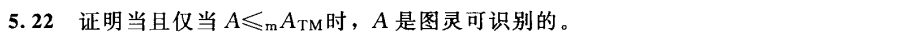
\includegraphics[width=0.8\textwidth]{chapters/imgs/hw_5_22.png}
  \caption{}
  \label{fig:hw_5_22}
\end{figure}

答案：$X$ 不可判定。

\medskip
证明。反设存在图灵机 $R$ 判定
\[
    X.
\]
我们构造图灵机 $S$ 来判定
\[
    A_{\mathrm{TM}}
\]
如下。给定输入
\[
    \langle M,w\rangle,
\]
$S$ 构造一台单带图灵机 $N$，并把固定输入串 $0$ 交给 $R$ 检查。

\begin{myalgo}{构造的单带图灵机 $N$}
\begin{algorithmic}[1]
  \Require 任意输入
  \Ensure 仅当 $M$ 接受 $w$ 时修改原输入区域
  \State 向右移动到初始输入区域之后的第一个空白格
  \State 从该空白格开始，只在输入区域右边模拟 $M$ 在输入 $w$ 上的计算
  \If{模拟发现 $M$ 接受 $w$}
    \State 返回输入区域，并改写其最左端输入符号，然后接受
  \ElsIf{$M$ 拒绝 $w$}
    \State \textbf{拒绝}
  \Else
    \State 在右侧工作区继续循环
  \EndIf
\end{algorithmic}
\end{myalgo}

\begin{myalgo}{构造的图灵机 $S$}
\begin{algorithmic}[1]
  \Require 输入 $\langle M,w\rangle$
  \Ensure 若 $\langle M,w\rangle\in A_{\mathrm{TM}}$ 则接受；否则拒绝
  \State 构造上述单带图灵机 $N$
  \State 在输入 $\langle N,0\rangle$ 上运行 $R$
  \If{$R$ 接受}
    \State \textbf{拒绝}
  \Else
    \State \textbf{接受}
  \EndIf
\end{algorithmic}
\end{myalgo}

\medskip
下面验证正确性。若
\[
    \langle M,w\rangle\in A_{\mathrm{TM}},
\]
则 $N$ 最终会改写输入串 $0$ 所在的那一段输入区域，所以
\[
    \langle N,0\rangle\notin X.
\]
于是 $R$ 拒绝，$S$ 接受。

\medskip
若
\[
    \langle M,w\rangle\notin A_{\mathrm{TM}},
\]
则 $N$ 永远不会改写输入区域，因此
\[
    \langle N,0\rangle\in X.
\]
于是 $R$ 接受，$S$ 拒绝。

\medskip
因此 $S$ 判定了
\[
    A_{\mathrm{TM}},
\]
矛盾。

故 $X$ 不可判定。$\blacksquare$

\paragraph{解释.}
题目问的是一个“具体输入上的运行行为”，不是语言性质，所以不能直接套 Rice 定理。但 reduction 很直接：让机器先把真正的模拟全部放到输入右边，只在“模拟成功”时才回头碰原输入。于是“会不会修改输入区”就等价于“$M$ 会不会接受 $w$”。

\subsection*{5.24}

\begin{figure}[H]
  \centering
  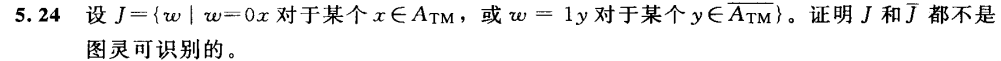
\includegraphics[width=0.8\textwidth]{chapters/imgs/hw_5_24.png}
  \caption{}
  \label{fig:hw_5_24}
\end{figure}

\paragraph{(a)}
证明。设
\[
    G=(V,\Sigma,R,S)
\]
是一部 CFG，规则集为
\[
    R=\{r_1,\dots,r_m\}.
\]
对每条规则 $r_i$，记
\[
    G_i=(V,\Sigma,R\setminus\{r_i\},S).
\]

构造识别器 $T$ 来识别 $\mathrm{MIN}_{\mathrm{CFG}}$。在输入 $\langle G\rangle$ 上，$T$ 并行地对每个 $i=1,\dots,m$ 搜索一个见证串 $w_i$，满足
\[
    w_i\in L(G)\setminus L(G_i).
\]

更具体地，$T$ 交错枚举所有字符串
\[
    w_1,w_2,w_3,\dots
\]
并对每条规则 $r_i$ 同时进行如下测试：寻找某个字符串 $w$，使得
\[
    w\in L(G)
    \qquad\text{且}\qquad
    w\notin L(G_i).
\]
由于 CFG 成员资格问题可判定，这两个测试都能停机。

\medskip
若 $G$ 是最小的，则删除任意一条规则都会改变语言。因此对每个 $i$ 都存在某个见证串 $w_i$，于是上述搜索最终会为每条规则都找到见证，机器 $T$ 接受。

\medskip
反之，若 $G$ 不是最小的，则存在某条规则 $r_j$ 满足
\[
    L(G_j)=L(G).
\]
于是对该 $j$ 而言，不存在见证串
\[
    w\in L(G)\setminus L(G_j),
\]
所以搜索永远不会结束，$T$ 也不会接受。

\medskip
因此 $T$ 恰好识别 $\mathrm{MIN}_{\mathrm{CFG}}$。故 $\mathrm{MIN}_{\mathrm{CFG}}$ 是 Turing-recognizable 的。$\blacksquare$

\paragraph{(b)}
证明。利用前一题 5.23(b) 的结论：语言
\[
    \mathrm{NECESSARY}_{\mathrm{CFG}}
    =\{\langle G,A\rangle\mid A\text{ 是 }G\text{ 的必要变量}\}
\]
是不可判定的。反设存在图灵机 $R$ 判定
\[
    \mathrm{MIN}_{\mathrm{CFG}}.
\]
我们构造图灵机 $S$ 来判定
\[
    \mathrm{NECESSARY}_{\mathrm{CFG}}.
\]

\medskip
给定输入
\[
    \langle G,A\rangle,
\]
构造一个新文法 $H$。做法是：引入新变量 $A_0$，把 $G$ 中右部出现的每个 $A$ 都替换成 $A_0$，并加入唯一的桥接规则
\[
    A_0\to A.
\]
若原来的开始变量就是 $A$，则再引入新的开始变量 $S_0$，令
\[
    S_0\to A_0;
\]
否则开始变量保持不变。

\medskip
这样构造后，$H$ 与 $G$ 生成同一语言，但 $H$ 中一切对变量 $A$ 的使用都必须经过这条桥接规则
\[
    A_0\to A.
\]
因此，删除这条规则后，恰好相当于“禁止一切含有 $A$ 的推导”。

\medskip
于是
\[
    A\text{ 是 }G\text{ 的必要变量}
    \iff
    A_0\to A\text{ 是 }H\text{ 的必要规则}.
\]
换言之，
\[
    A\text{ 必要}
    \iff
    \text{删去 }A_0\to A\text{ 会改变 }H\text{ 的语言}.
\]

\medskip
最后，对 $H$ 的其余规则加上标准的 witness-padding：为每一条非桥接规则附加一个只通过该规则才能生成的私有见证串。这样做不影响上面这条桥接规则是否可删，但会保证所有其他规则都自动成为必要规则。于是得到的新文法 $\widehat H$ 满足
\[
    \widehat H\in \mathrm{MIN}_{\mathrm{CFG}}
    \iff
    A\text{ 是 }G\text{ 的必要变量}.
\]

于是定义
\begin{myalgo}{构造的图灵机 $S$}
\begin{algorithmic}[1]
  \Require 输入 $\langle G,A\rangle$
  \Ensure 若 $A$ 是 $G$ 的必要变量则接受；否则拒绝
  \State 按上述步骤构造文法 $\widehat H$
  \State 在输入 $\langle \widehat H\rangle$ 上运行 $R$
  \If{$R$ 接受}
    \State \textbf{接受}
  \Else
    \State \textbf{拒绝}
  \EndIf
\end{algorithmic}
\end{myalgo}

\medskip
由
\[
    \widehat H\in \mathrm{MIN}_{\mathrm{CFG}}
    \iff
    A\text{ 是 }G\text{ 的必要变量}
\]
可知，$S$ 判定了
\[
    \mathrm{NECESSARY}_{\mathrm{CFG}},
\]
矛盾。故
\[
    \mathrm{MIN}_{\mathrm{CFG}}
\]
不可判定。$\blacksquare$

\paragraph{解释.}
(a) 的思路很直接：最小文法的定义本身就是“每条规则都能找到一个删掉后失去的见证串”。(b) 的关键是把“变量 $A$ 是否必要”压缩成“一条桥接规则是否必要”，然后用标准 padding 技巧把别的规则都强制成必要的，于是最小性就只剩下这一条规则在起作用。

\subsection*{5.28}

\begin{figure}[H]
  \centering
  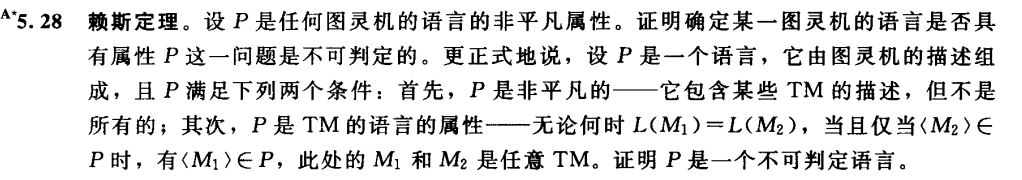
\includegraphics[width=0.8\textwidth]{chapters/imgs/hw_5_28.png}
  \caption{}
  \label{fig:hw_5_28}
\end{figure}

设
\[
    \mathrm{BLANKWRITE}
    =
    \{\langle M\rangle\mid M\text{ 是单带 TM，且在某个输入上曾把一个非空白符改写为空白符}\}.
\]

证明 $\mathrm{BLANKWRITE}$ 不可判定。反设存在图灵机 $R$ 判定
\[
    \mathrm{BLANKWRITE}.
\]
我们构造图灵机 $S$ 来判定
\[
    A_{\mathrm{TM}}
\]
如下。给定输入
\[
    \langle M,w\rangle,
\]
$S$ 构造一台单带图灵机 $N$：

\begin{myalgo}{构造的单带图灵机 $N$}
\begin{algorithmic}[1]
  \Require 任意输入
  \Ensure 仅当 $M$ 接受 $w$ 时发生“把非空白改写为空白”
  \State 忽略外部输入，先在带上某个固定位置写下一个非空白符，例如 $1$
  \State 模拟 $M$ 在输入 $w$ 上的运行
  \If{模拟发现 $M$ 接受 $w$}
    \State 回到第 1 步写下的那个 $1$，把它改写成空白符，再接受
  \ElsIf{$M$ 拒绝 $w$}
    \State \textbf{拒绝}
  \Else
    \State 继续循环
  \EndIf
\end{algorithmic}
\end{myalgo}

\begin{myalgo}{构造的图灵机 $S$}
\begin{algorithmic}[1]
  \Require 输入 $\langle M,w\rangle$
  \Ensure 若 $\langle M,w\rangle\in A_{\mathrm{TM}}$ 则接受；否则拒绝
  \State 构造上述单带图灵机 $N$
  \State 在输入 $\langle N\rangle$ 上运行 $R$
  \If{$R$ 接受}
    \State \textbf{接受}
  \Else
    \State \textbf{拒绝}
  \EndIf
\end{algorithmic}
\end{myalgo}

\medskip
下面验证正确性。若
\[
    \langle M,w\rangle\in A_{\mathrm{TM}},
\]
则 $M$ 接受 $w$，于是 $N$ 在某次计算中会把先前写下的非空白符擦成空白，因此
\[
    \langle N\rangle\in \mathrm{BLANKWRITE},
\]
从而 $R$ 接受，$S$ 接受。

\medskip
若
\[
    \langle M,w\rangle\notin A_{\mathrm{TM}},
\]
则这种改写永不发生，所以
\[
    \langle N\rangle\notin \mathrm{BLANKWRITE},
\]
从而 $R$ 拒绝，$S$ 拒绝。

\medskip
因此 $S$ 判定了
\[
    A_{\mathrm{TM}},
\]
矛盾。故 $\mathrm{BLANKWRITE}$ 不可判定。$\blacksquare$

\paragraph{解释.}
这是一个很典型的“先埋一个记号，再决定是否擦掉它”的 reduction。题目问“是否曾经发生过某种写带行为”，就把这次行为安排成“只在原问题答案为 yes 时发生”即可。

\subsection*{5.33}

\begin{figure}[H]
  \centering
  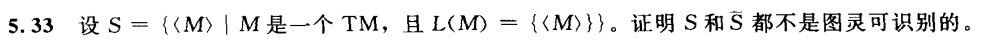
\includegraphics[width=0.8\textwidth]{chapters/imgs/hw_5_33.png}
  \caption{}
  \label{fig:hw_5_33}
\end{figure}

证明。设 PCP 的字母表为一元字母表
\[
    \Sigma=\{1\}.
\]
于是每个牌
\[
    \langle t_i,b_i\rangle
\]
实际上只由两个正整数
\[
    m_i=|t_i|,
    \qquad
    n_i=|b_i|
\]
决定，因为
\[
    t_i=1^{m_i},
    \qquad
    b_i=1^{n_i}.
\]

\medskip
对任意牌序列
\[
    i_1,\dots,i_k,
\]
其顶部和底部拼接结果相同，当且仅当
\[
    m_{i_1}+\cdots+m_{i_k}
    =
    n_{i_1}+\cdots+n_{i_k}.
\]
等价地，
\[
    (m_{i_1}-n_{i_1})+\cdots+(m_{i_k}-n_{i_k})=0.
\]

\medskip
因此，一元字母表上的 PCP 是否有解，只取决于整数集合
\[
    d_i=m_i-n_i.
\]
现在分情况讨论：

\medskip
\noindent
1. 若某个 $d_i=0$，则单独选这块牌就得到一个解。

\medskip
\noindent
2. 若存在
\[
    d_i>0
    \quad\text{且}\quad
    d_j<0,
\]
则也一定有解。因为取
\[
    |d_j|
\]
张第 $i$ 块牌和
\[
    d_i
\]
张第 $j$ 块牌，就有
\[
    |d_j|d_i+d_i d_j=0.
\]
于是可得到顶部与底部总长度相等的拼接。

\medskip
\noindent
3. 若所有 $d_i$ 都严格为正，或都严格为负，则任意非空牌序列的总差也严格为正或严格为负，不可能为 $0$，因而无解。

\medskip
所以，一个一元 PCP 实例有解，当且仅当满足以下二者之一：

\medskip
\noindent
1. 某个 $d_i=0$；

\medskip
\noindent
2. 同时存在正的 $d_i$ 和负的 $d_j$。

\medskip
这是一个显然可判定的有限检查过程。故 PCP 在一元字母表上是可判定的。$\blacksquare$

\paragraph{解释.}
一旦字母表只剩下
\[
    1,
\]
串本身就不再携带结构信息，唯一重要的只是长度。于是 PCP 退化成一个整数平衡问题：能不能把若干个差值
\[
    d_i=|t_i|-|b_i|
\]
相加得到 $0$。这在一元情形下就完全变成了有限算术判断。

\clearpage
